\section{Results} \label{sec:results}
Our goal in this paper is to infer the posterior of cosmological parameters
$\Omega = \{ \Omega_m, \sigma_8 \}$ and baryonic feedback parameters 
$\mathcal{B} = \{ A_{\rm SN1}, A_{\rm SN2}, A_{\rm AGN1}, A_{\rm AGN2}\}$ from the observed photometry
of galaxies in the NSA catalog, $\{\bfi X_i\}$: 
$p(\Omega, \mathcal{B} \given \{{\bfi X_i}\})$.
We graphically represent our approach in Figure~\ref{fig:graph}.
Circles, shaded circles, and dots represent random variables, observed
quantities, and random variables that are deterministic. 
$\theta_i^g$, the physical properties of galaxies (\emph{e.g.} $M_*$,
star-formation history), are determined from $\Omega$ and $\mathcal{B}$ through
the hydrodynamical models used to construct CAMELS.
Then the photometry $X_i$ is determined from $\theta_i^g$ through the SED model
based on stellar population synthesis (Section~\ref{sec:sim}).  

\begin{figure}
\begin{center}
    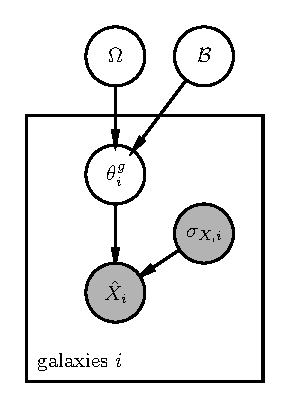
\includegraphics[width=0.4\textwidth]{figs/graph.pdf} 
    \caption{
        Graphical representation of our hierarchical approach that illustrate
        the relationship among the main parameters of our model. 
        Circles are inferred random variables, shaded circles are observed
        quantities, and dots indicate random variables that are deterministic.
    }\label{fig:graph}
\end{center}
\end{figure}


Given this hierarchical model, we can rewrite the posterior of interest: 
\begin{align}
p(\Omega, \mathcal{B} \given \{{\bfi X_i}\}) 
    =&~\frac{p(\Omega, \mathcal{B})~p(\{{\bfi X_i}\} \given \Omega, \mathcal{B})}{p(\{{\bfi X_i}\})}\\
    =&~\frac{p(\Omega, \mathcal{B})}{p(\{{\bfi X_i}\})}\int p(\{{\bfi X_i}\}
    \given \{\theta^g_i\})~p(\{\theta^g_i\} \given \Omega, \mathcal{B})~{\rm d}\{\theta^g_i\}.\\
    =&~\frac{p(\Omega, \mathcal{B})}{p(\{{\bfi X_i}\})}\prod\limits_{i=1}^N\int
    p({\bfi X_i} \given \theta^g_i)~p(\theta^g_i \given \Omega, \mathcal{B})~{\rm d}\theta^g_i\\
    =&~\frac{p(\Omega, \mathcal{B})}{p(\{{\bfi X_i}\})}\prod\limits_{i=1}^N\int
    \frac{p(\theta^g_i \given {\bfi X_i})~p({\bfi
    X_i})}{p(\theta^g_i)}~p(\theta^g_i \given \Omega, \mathcal{B})~{\rm d}\theta^g_i\\
    =&~p(\Omega, \mathcal{B})\prod\limits_{i=1}^N\int \frac{~p(\theta^g_i
    \given \Omega, \mathcal{B})}{p(\theta^g_i)} p(\theta^g_i \given {\bfi X_i})
    ~{\rm d}\theta^g_i\\
    =&~p(\Omega, \mathcal{B})\prod\limits_{i=1}^N\int \frac{p(\Omega, \mathcal{B}\given \theta^g_i)}{p(\Omega, \mathcal{B})}
p(\theta^g_i \given {\bfi X_i})~{\rm d}\theta^g_i \\
     \label{eq:post0}
    =&~\frac{1}{p(\Omega, \mathcal{B})^{N-1}}\prod\limits_{i=1}^N\int p(\Omega,
    \mathcal{B}\given \theta^g_i) p(\theta^g_i \given {\bfi X_i})~{\rm
    d}\theta^g_i  \\
     \label{eq:posterior}
    =&~\frac{1}{p(\Omega, \mathcal{B})^{N-1}}\prod\limits_{i=1}^N p(\Omega,
    \mathcal{B}\given {\bfi X_i}).
\end{align} 
With Eq.~\ref{eq:posterior}

explain that $\theta^g$ are latent variables. 


%\intertext{
%    We estimate the integral using $S_i$ Monte Carlo samples from the
%    individual posteriors $p(\theta^g_i \given {\bfi X_i})$: 
%}
%    \approx&~\frac{1}{p(\Omega, \mathcal{B})^{N-1}}\prod\limits_{i=1}^N\frac{1}{S_i}\sum\limits_{j=1}^{S_i} p(\Omega, \mathcal{B} \given \theta^g_{i,j}).
